\ifreview
Comments to address in this section:
\begin{enumerate}
    \color{red} 
    
    \item REVIEWER 2: What are the reasons for the low efficiency of PanDA
    Broker? Why are only 30\% of backfill slots useable, if they are basically
    uncontested? \jhanote{MT to address this via a few sentences in Section
    IV.}
    
    % \item REVIEWER 2: Why does Fig 3 show an increase of absolute and
    % relative efficiency in Aug-16, when the text claims this in Sep-16 due to
    % more PanDA Brokers?\mtnote{Fixed.}
    
    % \item REVIEWER 2: Why are only 20 PanDA Brokers deployed if this is a
    % limiting factor? Why is it questionable that more PanDA Brokers would
    % increase efficiency? If only 5/6 of resources below the mean are
    % unusable, this implies an efficiency of almost 60\% being
    % reachable.\mtnote{From our text: ``further research is ongoing to
    % understand whether an even greater number of brokers would yield even
    % greater efficiency. This research focuses on evaluating the overheads of
    % input/output files staging, including its impact on DTNs, and on an
    % alternative design of PanDA Broker that enables the concurrent submission
    % of multiple MPI scripts''. I believe this is an answer good enough.}

    % \item REVIEWER 2: Given an expected increase in resource need of 10-100,
    % how is the capacity of 4\% WLCG significant? How does this relate to the
    % manpower required to develop and maintain a custom solution per HPC site?
    % How many TITAN resources are actually available to HEP, given the use by
    % other domains? The magnitude of capacities presented as available is in
    % major contrast to the requirements sketched in the introduction.


    
    % \item REVIEWER 2: How does the poor metadata read performance of
    % 1500-6300s (25\%-100\% of minimum walltime!) affect efficiency? Is it
    % factored into the choice of walltime requests?\mtnote{Thanks to Sergey's
    % input I corrected the figure previously reported.} Is it applicable only
    % to TITAN, to HPC in general, or even to regular WLCG sites?\mtnote{This
    % is clearly out of scope for this paper.} Are there solutions at
    % application, e.g. the use of packaged python scripts and
    % libraries?\mtnote{Added the following: ``While these figures are specific
    % to OLCF and TItan, reengineering on AthenaMP could further improve
    % startup time on every platform.''} The information presented is
    % insufficient to estimate whether this issue applies to other environments
    % and usecases as well, or is simply due to suboptimal
    % implementation/configuration.
    
    % \item REVIEWER 3: The HEP-SPEC06 benchmark, which is used as a
    % ``computing power'' measure in LCG is mostly integer-artihmetic based: FP
    % operations accounts for \~10\% of the average workload (see [1], section
    % ``Why do you use `all\_cpp' instead of SPECint or SPECfp?'') While this
    % figure certainly comes from averaging over many different workloads
    % across all experiments, it seems a bit surprising that FP scheduling
    % contention is responsible for 50\% decrease in compute efficiency on
    % Titan when compared to other WLCG sites (paper page 6).\mtnote{Thanks to
    % Sergey's input I downplayed the role played by FP and up-played the role
    % played by new CPUs.}
\end{enumerate}
\fi

Currently 20 instances of the PanDA Broker are deployed on 4 DTNs, with
5 instances per DTN\@. Each broker submits and manages the execution of 15 to
300 jobs, one job for each Titan worker node, and a theoretical maximum
concurrent use of 96,000 cores. Since November 2015, PanDA Brokers have
operated only in backfill mode, without a defined time allocation, and
running at the lowest priority on Titan. Therefore, ATLAS contributed to an
increase of Titan's utilization.

We evaluate the efficiency, scalability and reliability of the deployment of
PanDA WMS on Titan by characterizing the behavior of both PanDA Broker and
AthenaMP\@. We discuss challenges and limitations of our approach at multiple
levels arising from the specifics of workload, middleware and methods. All
the measurements were performed between January 2016 and February 2017,
hereafter called `experiment time window'.

% ---------------------------------------------------------------------------
\subsection{Characterizing the PanDA Broker on Titan}\label{ssec:broker_titan}

We calculate the total amount of backfill availability over a period of time
by: (i) polling the available backfill slots at regular intervals during that
time window; (ii) converting the number of worker nodes available and their
walltime into core-hours; (iii) summing the number of core-hours. We call
this number of core-hours `total backfill availability'.

Fig.~\ref{fig:backfill-utilization} shows the total backfill availability on
Titan (gray bars) and the number of core-hours of that availability used by
ATLAS (blue bars) during the experiment time window. ATLAS consumed a total
of 51.4M core-hours, for an average of \(\approx\)3.7M core-hours a month.

\begin{figure}[!t]
    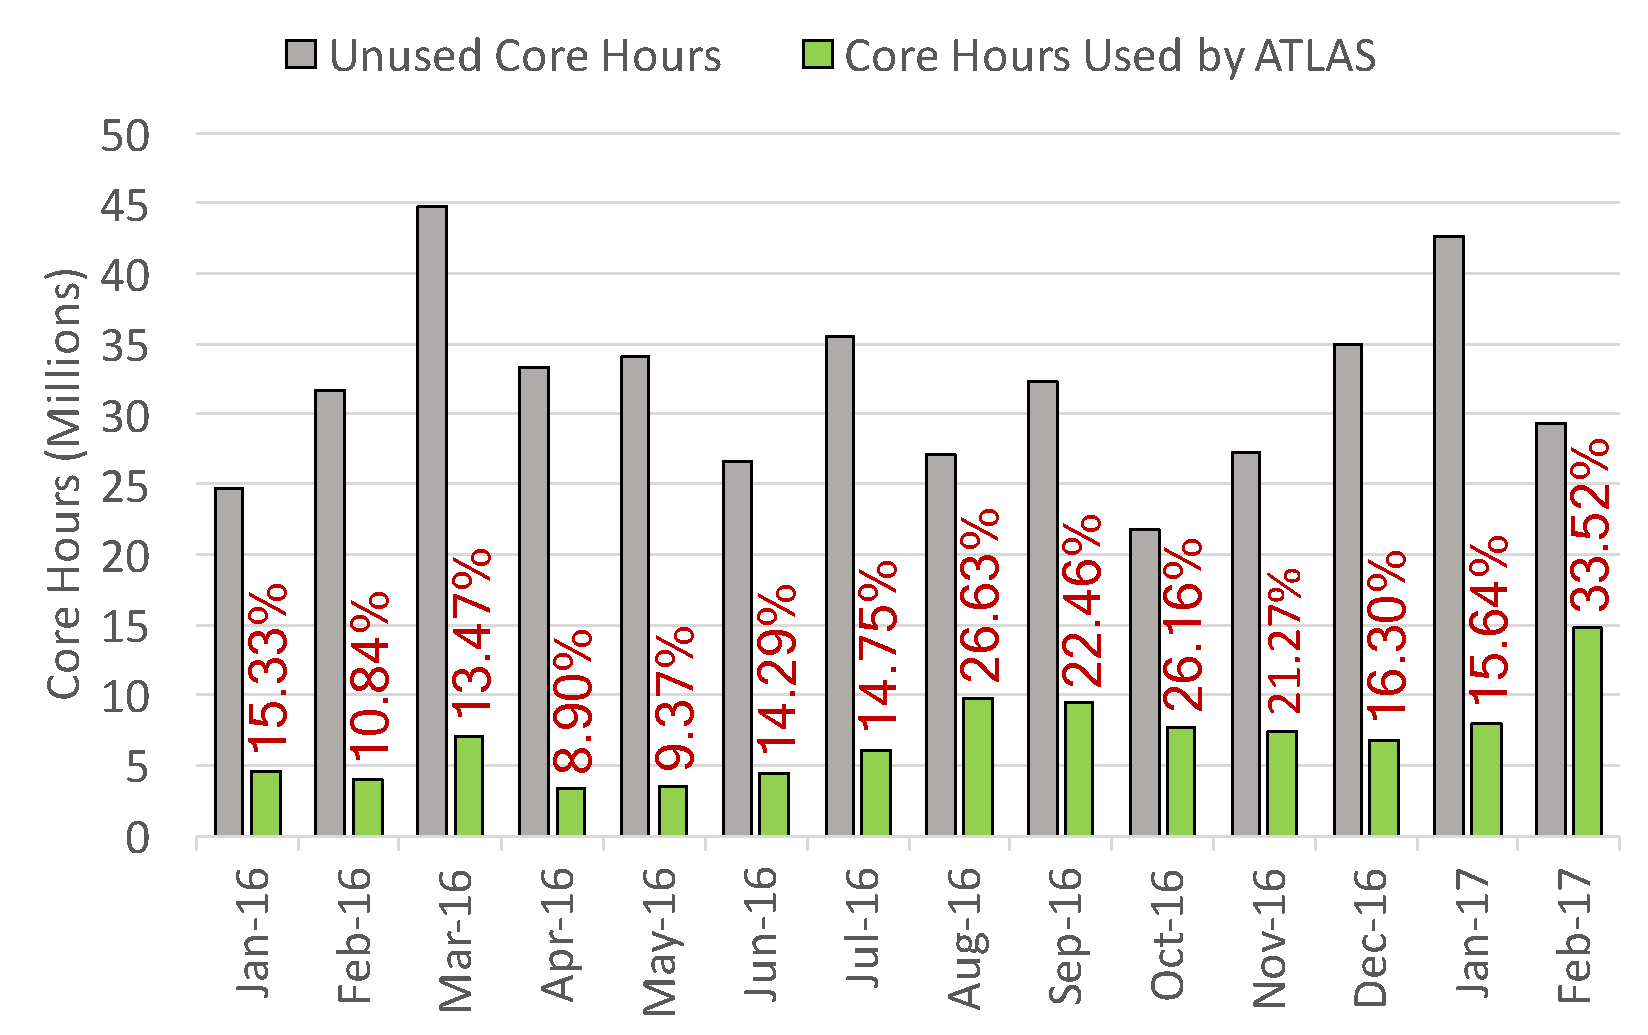
\includegraphics[clip,width=\columnwidth]{figures/backfill_consumption.pdf}
    \vspace{-0.3in}
    \caption{Titan's total backfill availability: CPU core-hours (gray) and
    CPU core-hours used by ATLAS (blue). GPU core-hours unaccounted for as
    they cannot be used by ATLAS\@. Efficiency of PanDA Brokers defined as
    percentage of total Titan's backfill availability used by ATLAS (Red
    labels).}\label{fig:backfill-utilization}
\end{figure}

PanDA Brokers' efficiency (Fig.~\ref{fig:backfill-utilization}, red labels) is
defined as the fraction (or percentage) of core-hours utilized by the PanDA
Brokers of Titan’s total backfill availability during the experiment time
window. The  average efficiency was 18\%, with a minimum efficiency
of 7.8\% (May 2016) and a maximum efficiency of 30.9\% (Feb. 2017, excluding
the preliminary results of March). The total backfill availability was
$\approx$ 21.5M in April 2016, and 17.6M in February 2017. This suggests that
the efficiency is invariant of total backfill availability.

% This suggests that the differences
% in efficiency did not depend on a comparable difference in the total backfill
% availability. 

% \jhanote{change last sentence to: ... efficiency does not depend on total
% backfill availability." ??}
% \jhanote{shouldn't we be consistent in the months used to quote efficiency and
% utilization? April 2016 and Feb 2017 vs May 2016 and Feb 2017??}

During the experiment time window, about 2.25M detector simulation jobs were
completed on Titan, for a total of 225M events processed. This is equivalent
to 0.9\% of all the 250M detector simulations performed by ATLAS in the same
period of time, and 3.5\% of the 6.6B events processed by those jobs. These
figures confirms the relevance of supercomputers' resource contribution to
the LHC Run 2, especially when accounting for the amount of unused total
backfill availability and the improvement of PanDA efficiency across the
experiment time window.

On February 2017, PanDA Brokers used almost twice as much total backfill
availability than in any other month (preliminary results for March 2017
displayed in Fig.~\ref{fig:backfill-utilization} confirm this trend). No
relevant code update was made during that period and logs indicated that the
brokers were able to perform faster. This is likely due to hardware upgrades
on the DTNs. The absence of continuous monitoring of those nodes does not
allow to quantify bottlenecks but spot measurements of their load indicate
that a faster CPU and better networking were likely responsible for the
improved performance. Investigations showed an average CPU load of 3.6\% on
the upgraded DTNs, as opposed to the ``high'' utilization reported by OLCF
for the previous DTNs. As such, further hardware upgrades seem unlikely to
improve significantly the performance of PanDA Brokers.\mtnote{Possibly, add
a small paragraph summarizing why at the moment we are consuming up to 30\%
of the available backfill.}

Every detector simulation executed on Titan process 100 events. This number
of events is consistent with the physics of the use case and with the average
duration of backfill availability. The duration of a detector simulation is a
function of the number of events simulated but not all events take the same
time to be simulated. One event simulation takes from \(\approx\)2 to
\(\approx\)40 minutes, with a mean of \(\approx\)14 minutes. Considering that
each worker node process up to 16 events concurrently, 100 events takes an
average of 105 minutes to process. As such, PanDA brokers do not use backfill
availability with less than 105 minutes walltime.

Fig.~\ref{fig:backfill-distrib} shows backfill availability on Titan as a
function of number of nodes and the time of their availability (i.e.,
walltime). We recorded these data by polling Titan's Moab scheduler at
regular intervals during the experiment window time. The mean number of nodes
was 691, and their mean walltime was 126 minutes. Detector simulations of 100
events, enable to use down to 5/6 of the mean walltime of backfill
availability. As such, it offers a good compromise for PanDA Broker
efficiency.

\begin{figure}[!t]
    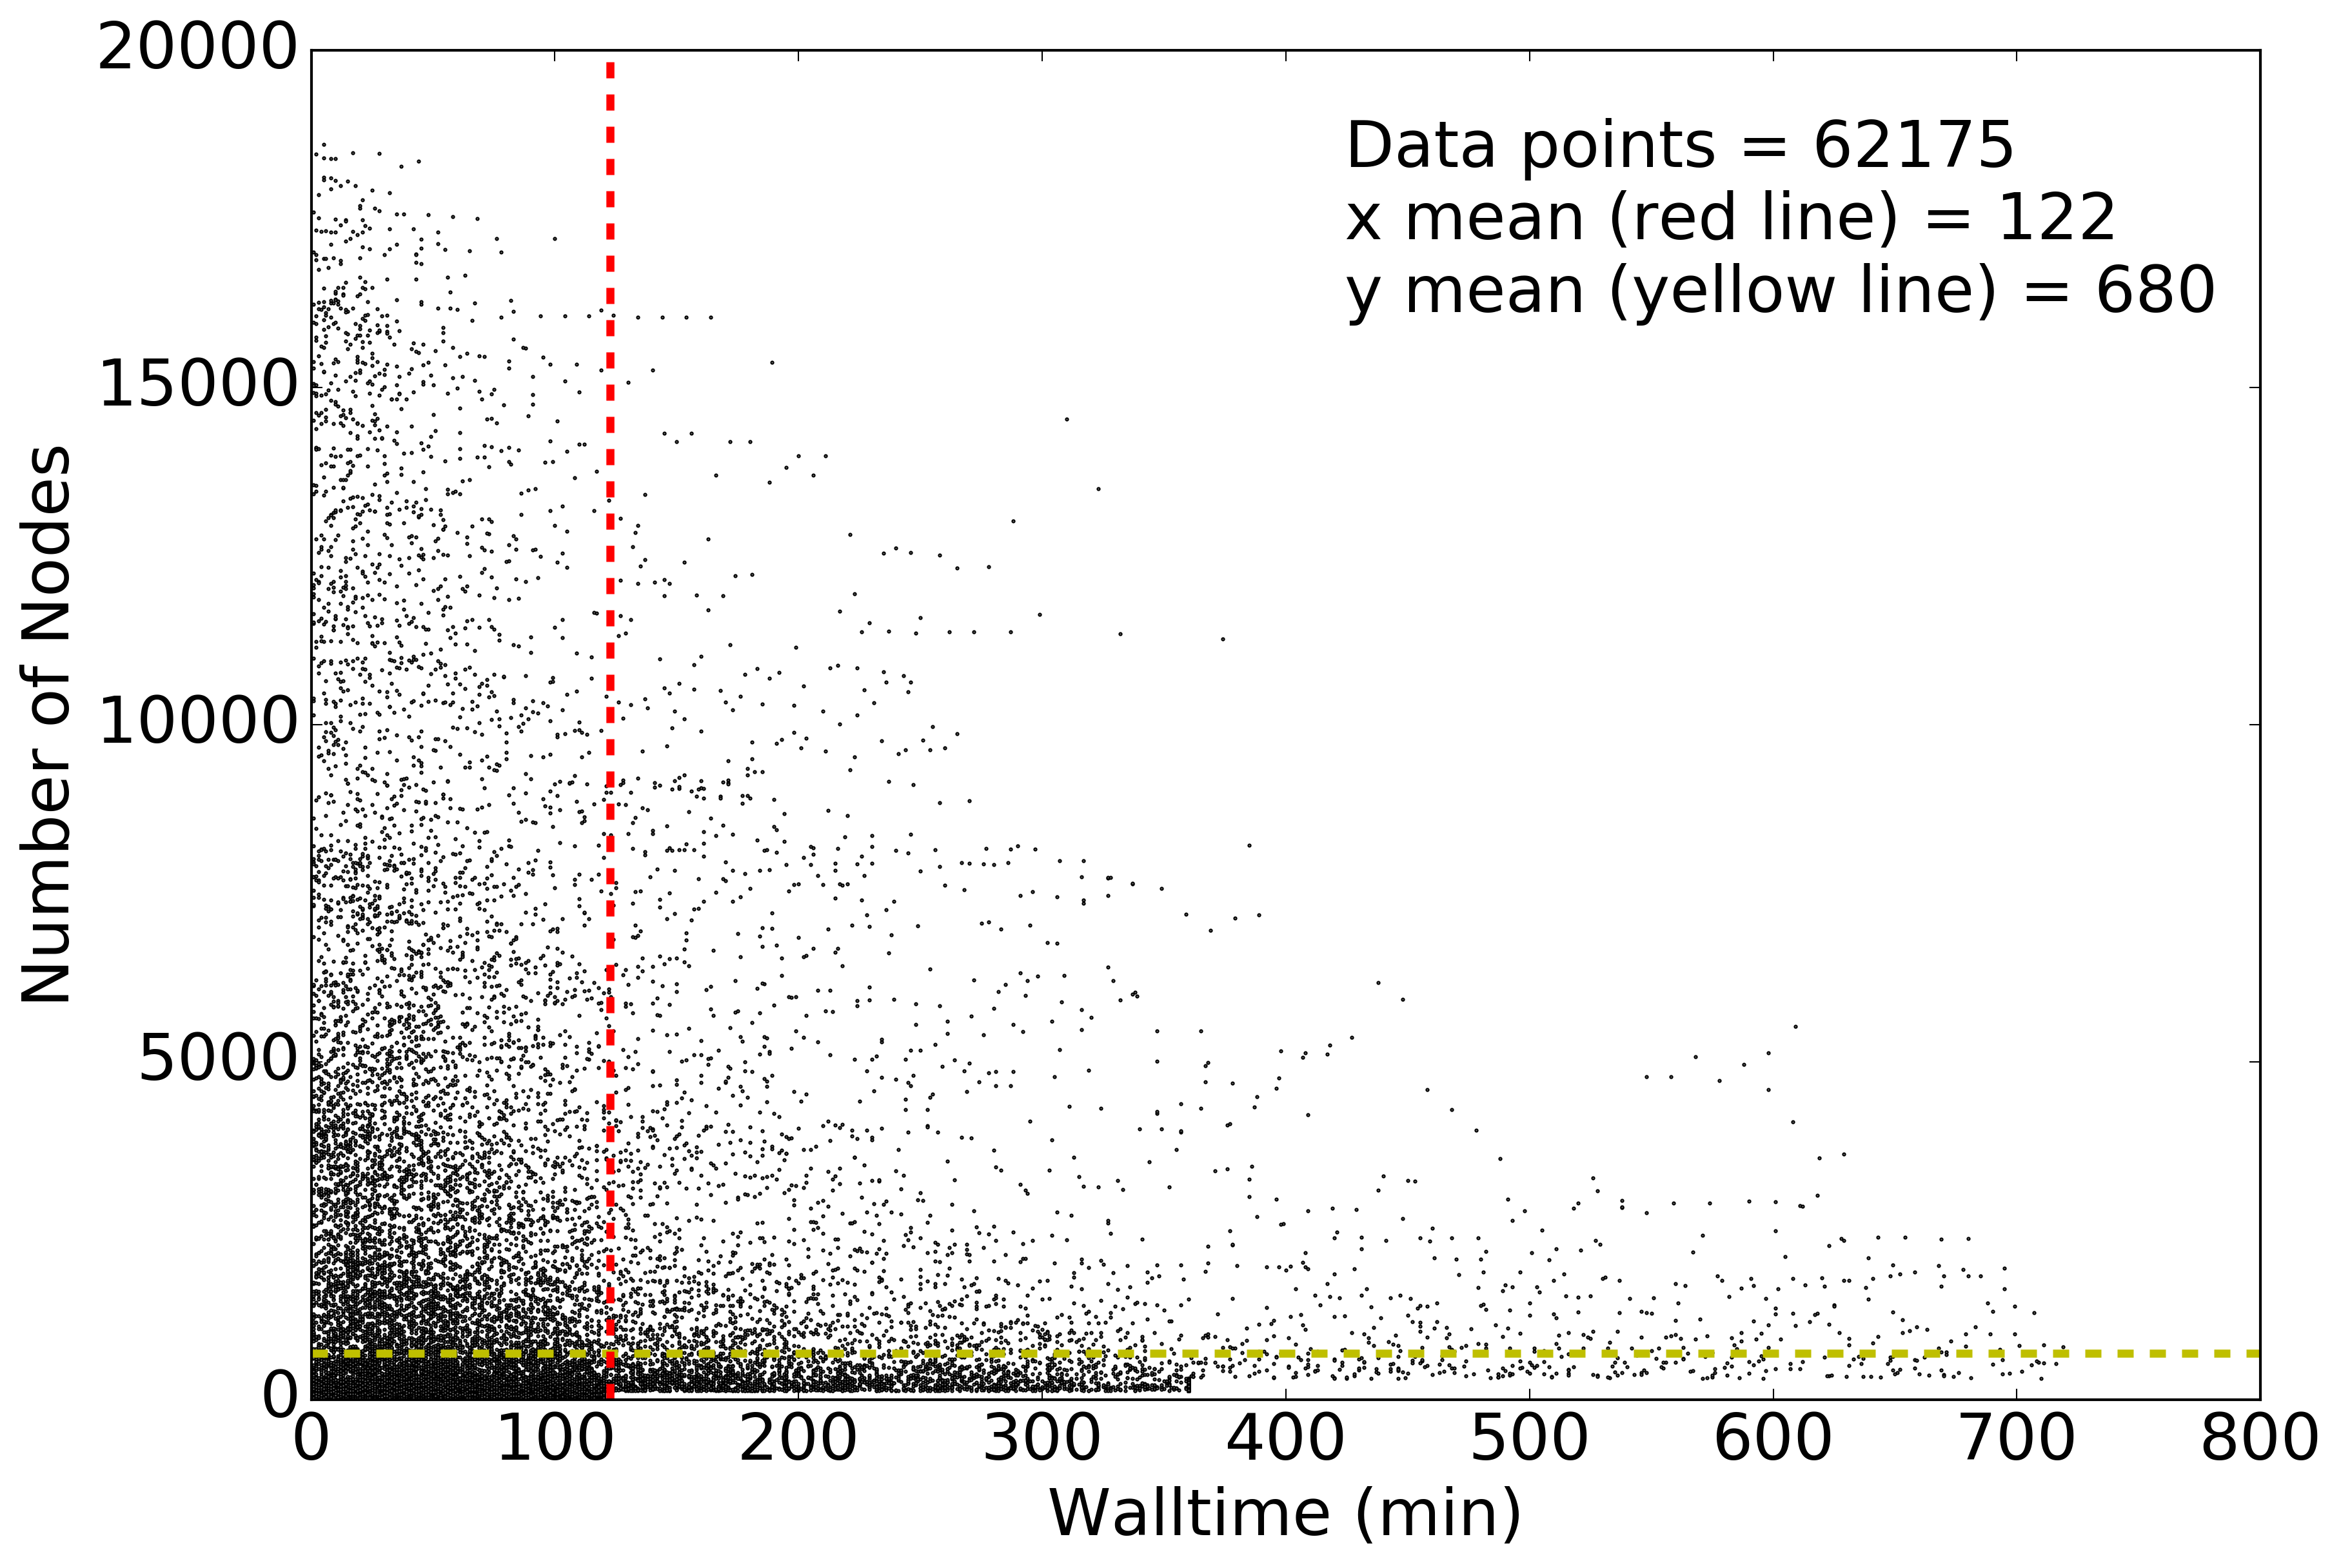
\includegraphics[clip,width=\columnwidth]{figures/titan_backfill_avail.png}
    \vspace{-0.1in}
    \caption{62555 measures of Backfill availability on Titan during the
    experiment time window. Mean number of work nodes available 691; mean
    walltime available 126 minutes.}\label{fig:backfill-distrib}
\end{figure}

PanDA Broker could fit the number of events to the walltime of each available
backfill slot on the base of the distributions of the time taken by one event
to be simulated. That specific number of event could then be pulled from the
PanDA Event service~\cite{calafiura2015atlas} and given as input to one or
more simulations. Once packaged into the MPI script submitted to titan's PBS
batch system, these simulations would better fit their available backfill
slot, contributing to increase the efficiency of PanDA Brokers.

The transition from a homogeneous to a heterogeneous number of events per
detector simulation has implications for the application layer. An even
number of events across simulations makes it easier to partition, track and
package events across simulations, especially when they are performed on both
the Grid and Titan. A homogeneous number of events also helps to keep the
size and duration of other stages of the MC workflow
(\S\ref{ssec:panda-titan}) more uniform. Further analysis is needed to
evaluate the trade offs between increased efficiency of resource utilization
and the complexity that would be introduced at the application layer.

Currently, each PanDA Broker creates, submits, and monitors a single MPI PBS
script at a time. This design is inherited from PanDA Pilot where a single
process is spawn at a time to execute the payload. As a consequence, the
utilization of a larger portion of Titan's total backfill availability
depends on the the number of concurrent PanDA Brokers instantiated on the
DTNs: When all the 20 PanDA Brokers have submitted a MPI PBS script, further
backfill availability cannot be used.

In August 2016, increasing the number of concurrent PanDA brokers from 4 to
20 markedly improved efficiency (see Fig.~\ref{fig:backfill-utilization}) but
further research is ongoing to understand whether an even greater number of
brokers would yield even greater efficiency. This research focuses on
evaluating the overheads of input/output files staging, including its impact
on DTNs, and on an alternative design of PanDA Broker that enables the
concurrent submission of multiple MPI scripts~\cite{barreiro2016panda}. The
understanding will contribute to improving the efficiency of PanDA Brokers
beyond the 30\% limit showed in Fig.~\ref{fig:backfill-utilization}.

The current design and architecture of the PanDA Broker is proving to be as
reliable as PanDA Pilot when used on the WLCG\@. Between Jan 2016 and Feb
2017, the overall failure rate of all the ATLAS detector simulation jobs was
14\%, while the failure rate of jobs submitted to Titan was a comparable
13.6\%. PanDA Brokers were responsible for around the 19\% of the failures,
compared to the 29\% of failures produced by the JobDispatcher module of the
PanDA Server, and the 13\% failures produced by the Geant4 toolkit. 

% ---------------------------------------------------------------------------
\subsection{Characterizing the Detector Simulation on
Titan}\label{ssec:athenamp_titan}

We use two main parameters to measure the performance of the detector
simulation jobs submitted to Titan: (i) the time taken to setup AthenaMP\@;
and (ii) the distribution of the time taken by Geant4 to simulate a certain
number of events.

AthenaMP has an initialization and configuration stage. At initialization
time, AthenaMP is assembled from a very large set of shared libraries,
depending on the type of payload that will have to be computed. Once
initialized, every algorithm and service of AthenaMP is configured via Python
scripts. Both these operations result in read operations on the filesystem
shared between the worker nodes and the DTNs, including the operations
required to access small python scripts.

Initially, all the shared libraries and the python scripts of AthenaMP were
stored on the OLCF Spider 2 Lustre file system. However, the I/O patterns of
the initialization and configuration stages degraded the performance of the
filesystem. This was addressed by moving the AthenaMP distribution to a
read-only NFS directory, shared among Titan's DTNs and worker nodes. NFS
eliminated the problem of metadata contention, improving metadata read
performance from a worse case scenario of 6,300s on Lustre to \(\approx\)225s
on NFS\@. While these figures are specific to OLCF and Titan, reengineering
of AthenaMP could improve startup time on every platform.

Once initialized and configured, AthenaMP is used to execute 16 concurrent
Geant4 simulators on a Titan's worker node. Geant4 requires to read events
descriptions from a filesystem and simulate them as they would happen within
the ATLAS detector. We characterized both the compute performance of the
simulation and the impact of acquiring event descriptions on the filesystem.

The AMD Opteron 6274 CPU used on Titan has 16 cores, divided into 8 compute
units. Each compute units has 1 floating point (FP) scheduler shared between
2 cores. When using 16 cores for FP-intensive calculations, each pair of
cores competes for a single FP scheduler. This creates the overhead shown in
Fig.~\ref{fig:comparison-8-16cores}: the mean runtime per event for 8
concurrent simulations computing 50 events is 10.8 minutes, while for 16
simulations is 14.25 minutes (consistent with the measured distribution of
the duration of event simulation). Despite an inefficiency of almost 30\%,
Titan's allocation policy based on number of worker nodes used instead of
number of cores does not justify the use of 1/2 of the cores available.

\begin{figure}[htp]
    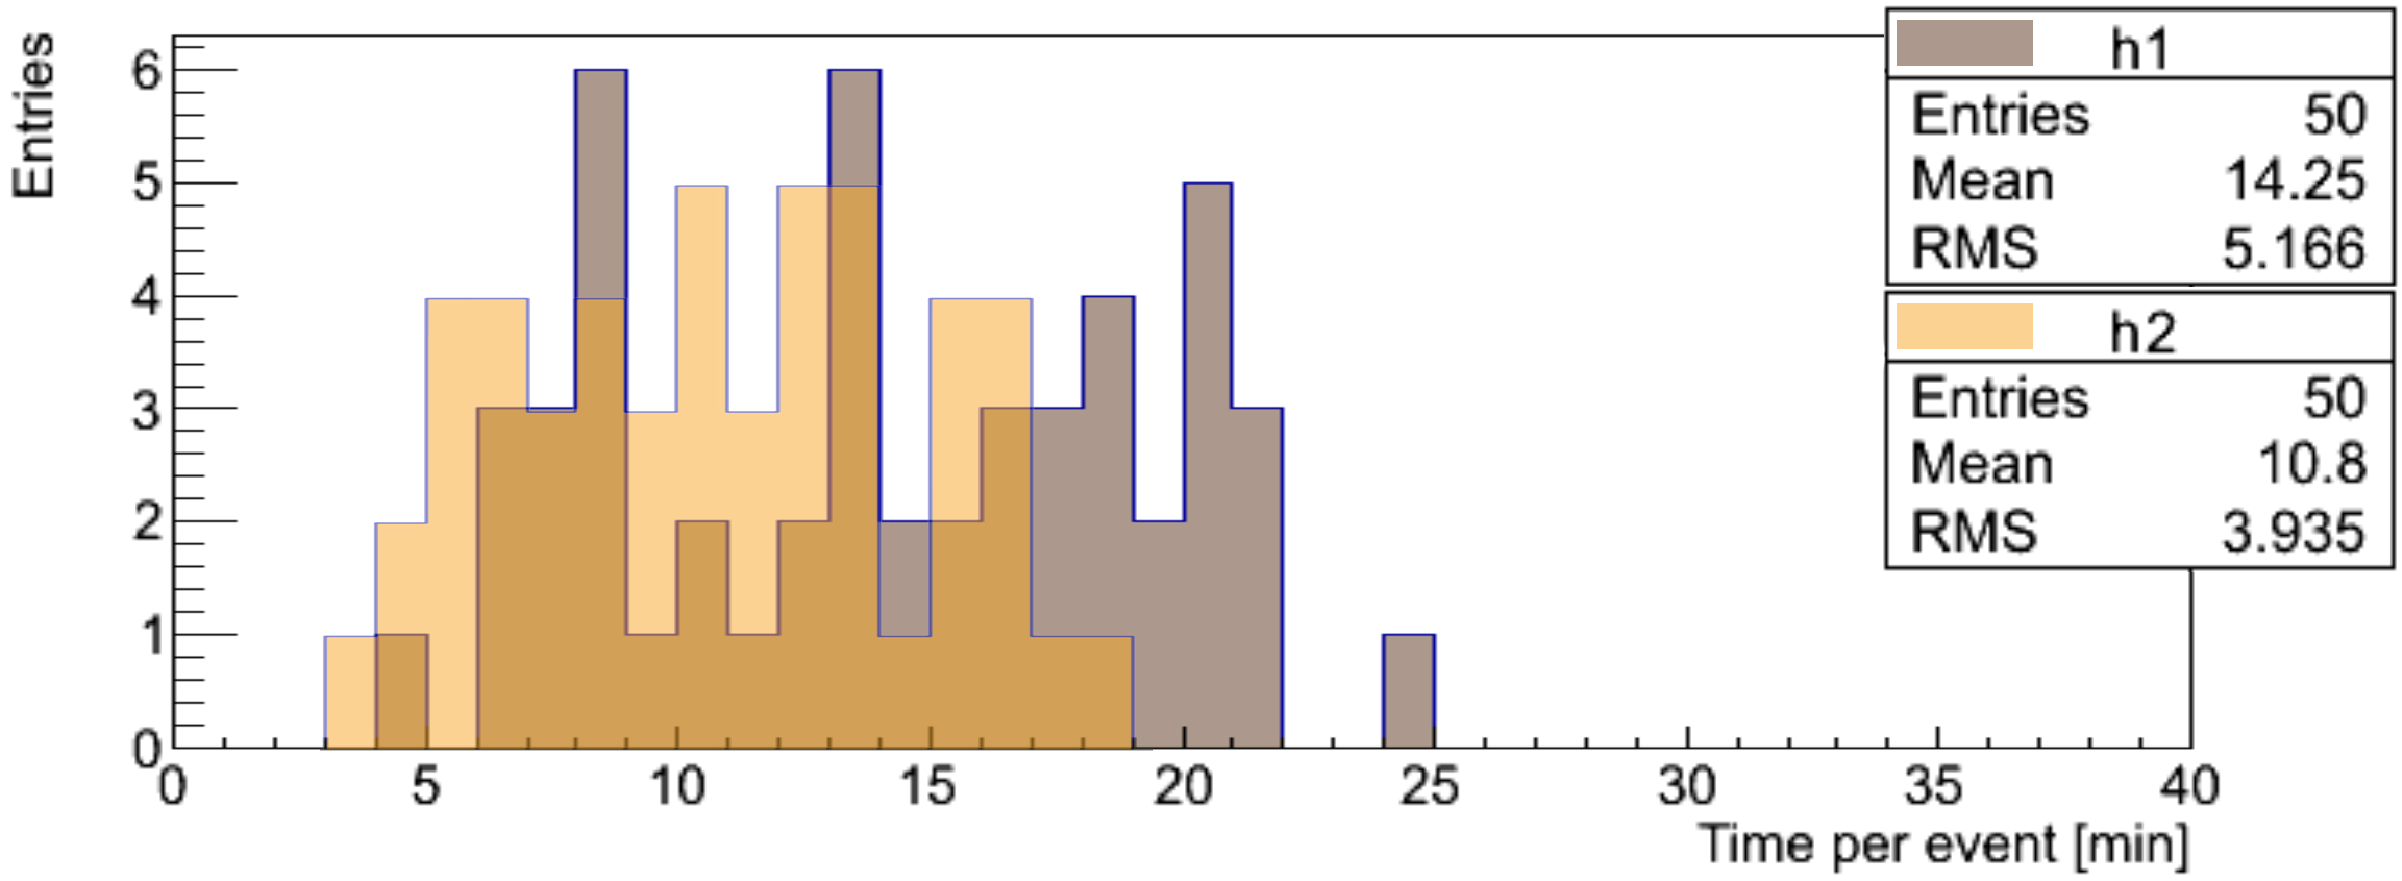
\includegraphics[clip,width=\columnwidth]{figures/tx8_tx16_comparison_vsquashed.pdf}
    \vspace{-0.3in}
    \caption{Distributions of the time taken to simulate one event when
    placing 2 simulations (h1) or 1 simulation (h2) per Titan's CPU\@. 2
    simulation use 16 cores per node, 1 simulation 8. 50 Events; 1 Titan
    worker nodes; 16 work threads per node; 100 events per
    node.}\label{fig:comparison-8-16cores}
\end{figure}

A performance analysis of Titan's AMD CPUs for detector simulations also helps
to compare Titan and Grid site performance. Usually, Grid sites expose
resources with heterogeneous CPU architectures and 8 (virtual) cores, while
Titan's offer an homogeneous 16 cores architecture. We used the rate of events
processes per minute as a measure of the efficiency of executing the same
detector simulation on Titan or Grid sites. Comparisons of the efficiencies of
Titan to the BNL and SIGNET Grid sites, normalized for 8 cores, show that the
effective performance per-core at Titan is
\(\approx\)0.57 event per minute, roughly 1/2 of BNL and  1/3 of SIGNET.

%performances.

% The CPUs at the Grid sites have one FP scheduler per core and are on
% average newer than the CPU of Titan.

The differences in performance between Titan and the BNL and SIGNET Grid
sites are due to the FP scheduler competition but mainly to the availability
of newer processors. 
The heterogeneity of the Grid sites' CPUs explain the higher performance
variance we observed compared to the performance consistency we measured on
Titan. This difference in performance is compensated by the amount of
resources available on Titan (capable of executing up to 30\%/year of the
ATLAS detector simulations) and by the lack of further resources available to
WLCG\@. Also, it should be noted that Titan is at the end of its life-cycle
and that Summit, Titan's successor, will offer cutting-edge performances.

We studied the impact of acquiring event descriptions on Lustre by analyzing
1,175 jobs ran on the week of 10/25/2016, for a total of 174 hours.
Table~\ref{panda-olcf-stats} shows the overall statistical breakdown of the
observed file I/O. ATLAS used between 1 and 300 worker nodes, and 35 on
average. 75\% of the jobs run by ATLAS consumed less than 25 nodes and 92\%
less than 100. During the 174 hours of data collection, 6.75 ATLAS jobs were
executed on average per hour, each job running for an average of 1.74 hours.
Every job read less than 250 GB and wrote less than 75 GB of data and, on
average, each job read 20 GB and wrote 6 GB of data.

\begin{table*}[t]
\centering
\begin{tabular}{lllllllll} & Num. Nodes & Duration (s) & Read (GB) & Written
 (GB) & GB Read/nodes & GB Written/nodes & \(open()\) & \(close()\) \\ Min & 1 &
 1,932 & 0.01 & 0.03 & 0.00037 & 0.02485 & 1,368 & 349 \\ Max & 300 & 7,452 &
 241.06 & 71.71 & 0.81670 & 0.23903 & 1,260,185 & 294,908 \\ Average & 35.66
 & 6,280.82 & 20.36 & 6.87 & 0.38354 & 0.16794 & 146,459.37 & 34,155.74 \\
 Std. Dev. & 55.33 & 520.99 & 43.90 & 12.33 & 0.19379 & 0.03376 & 231,346.55
 & 53,799.08
\end{tabular}
\caption{The Statistical breakdown of the I/O impact of 1,175 jobs ATLAS
executed at OLCF for the week of 10/25/16}\label{panda-olcf-stats}
\end{table*}

ATLAS jobs are read heavy: On average, the amount of data read per worker
node is less than 400 MB, while the amount of data written is less than 170
MB\@. Distributions of read and written data are different: The read
operation distribution per job shows a long tail, ranging from 12.5 GB to 250
GB, while the written amount of data has a very narrow distribution.

The metadata I/O breakdown shows that ATLAS jobs yield 23 file \(open()\)
operations per second (not including file \(stat()\) operations) and 5 file
\(close()\) operations per second, with similar distributions. On average,
the maximum number of file \(open()\) operations per job is \(\approx\)170/s
and the maximum number of file \(close()\) operations is \(\approx\)39/s. For
the 1,175 ATLAS jobs observed, the total number of file \(open()\) operations
is 172,089,760 and the total number of file \(close()\) operations is
40,132,992. The difference between these two values is under
investigation: a possible explanation is that ATLAS jobs don't call a file
\(close()\) operation for every file \(open()\) issued.

Overall, the average time taken to read events from input files stored on
Lustre is 1,320, comparable to the time taken to read the file required by
assembling AthenaMP from NFS\@. Preliminary investigation shows that this
time could be reduced to 40 seconds by loading the event descriptions into
the RAM disk available on each worker node. Events descriptions could be
transferred from Lustre to the RAM disk while configuring and initializing
AthenaMP, almost halving the time currently required by initiating a Geant4
simulation.